% Copyright (c) 2014,2016 Casper Ti. Vector
% Public domain.

\chapter{相关工作}  \label{chap:related}
\section{分布式数据库HBase}
HBase是Google BigTable\supercite{bigtable}的开源实现 ,是Hadoop 生态系统中一个列式NoSQL数据库,搭建在HDFS(Hadoop分布式文件系统)之上。HBase由于其优异的可扩展性和稳定性,在产业界得到了广泛应用。HBase也是图数据库Titan最常使用的存储引擎,为了介绍Titan的底层实现,此处先详述HBase的相关实现。
下面分别介绍HBase的数据模型、操作接口、存储实现以及HBase与同类系统的对比。

\subsection{HBase数据模型}
在HBase中,数据首先以表为单位进行组织。数据表以行为单位组织,每行由一个键值唯一标识,称为行键(row key)。一行中可以包含任意列的数据,每列对应的数据可分为多个版本(对应多个时间戳)。每个版本的数据是最小粒度的数据单元,称为一个单元格(cell)。因此一个单元格由行键、列名、版本号(时间戳)和值(value)组成。
在HBase中,各列按列族(column family)进行组织,因此列名实际由列族名和列修饰符(column qualifier)组成。区别于传统关系模型,列族里的列修饰符可以随时添加,不需要事先定义。即在插入数据时,可以指定任意的列修饰符。行键是每个表必须要有的一列,且只能是唯一的一列,不属于任何列族。图\ref{fig:hbase_table}是HBase中一张数据表的示例。

\begin{figure}[htbp]
\centering
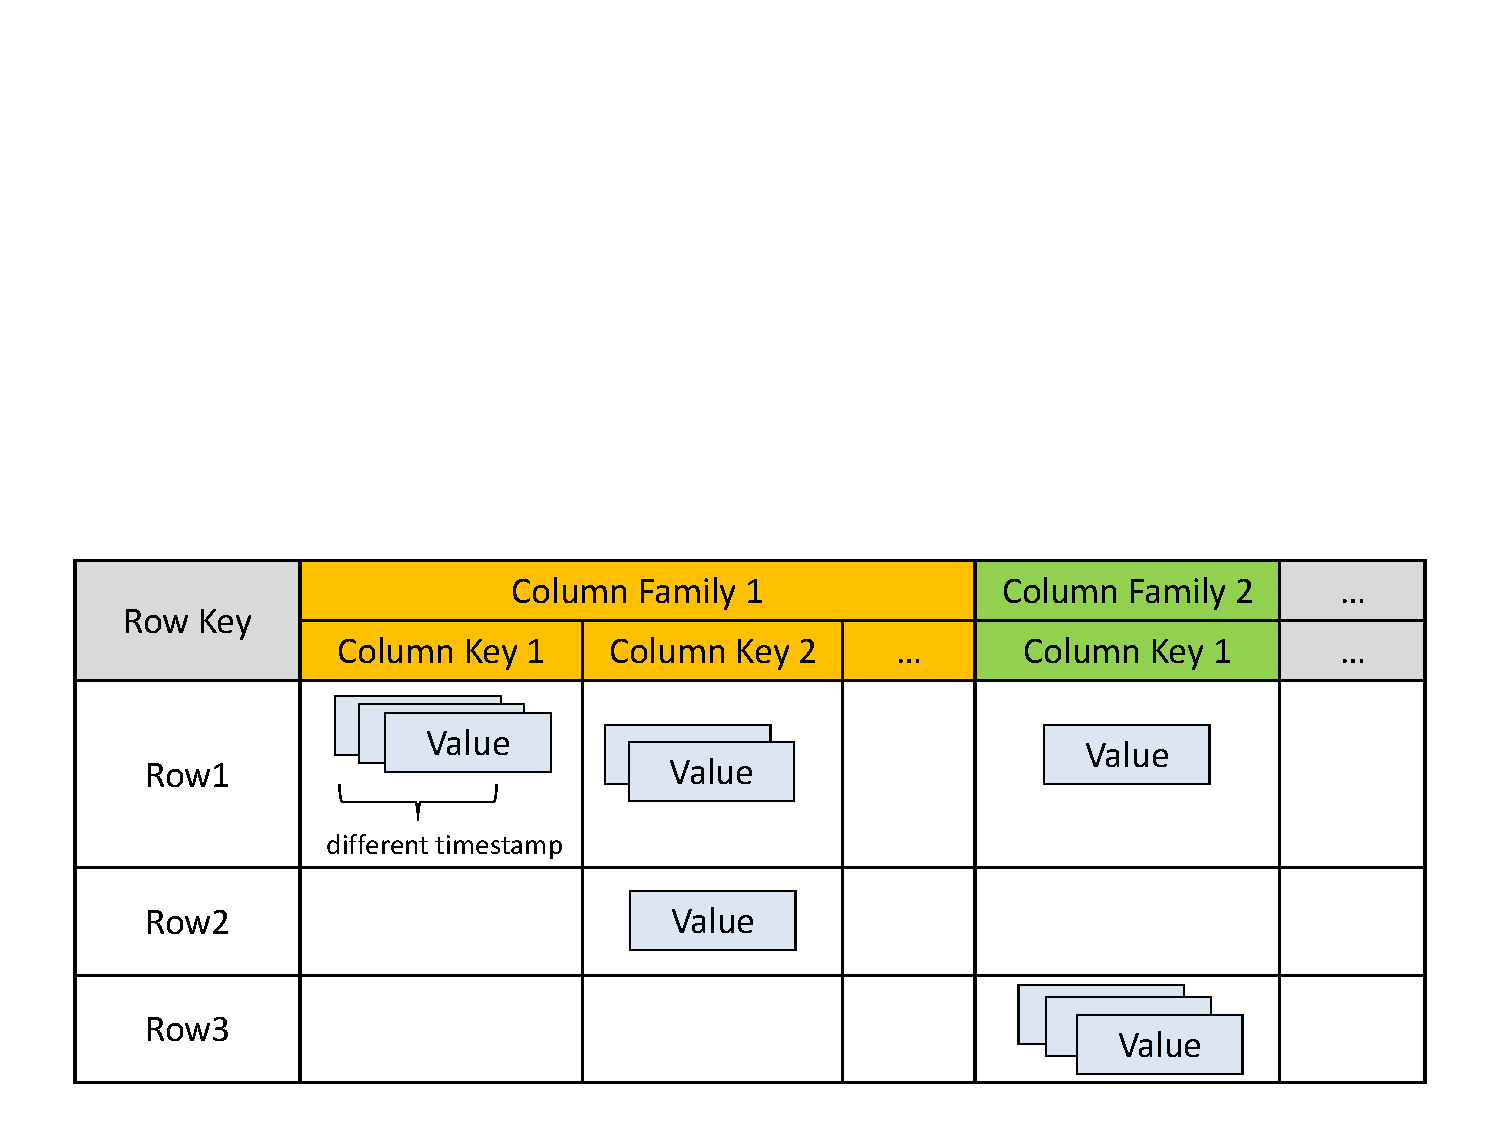
\includegraphics[width=120mm]{fig/HBase_table_example.pdf}
\caption{HBase数据表示例}
\label{fig:hbase_table}
\end{figure}

HBase也被认为是一个键值存储(Key-Value Store),相当于数据结构Map的存储。这是因为每个单元格实际存储的是Value部分,而Key部分就是由行键、列族名、列修饰符和时间戳合并构成。由于列修饰符是不需要事先定义的,因此整个Key部分是可以随意指定的,从而可以将HBase归类为键值存储。图\ref{fig:hbase_cell}是一个Cell的数据组成以及如何表示为键值对的示例。单元格也确实是HBase的存储实现中的最小单元,因此将HBase归类为键值存储。

\begin{figure}[htbp]
\centering
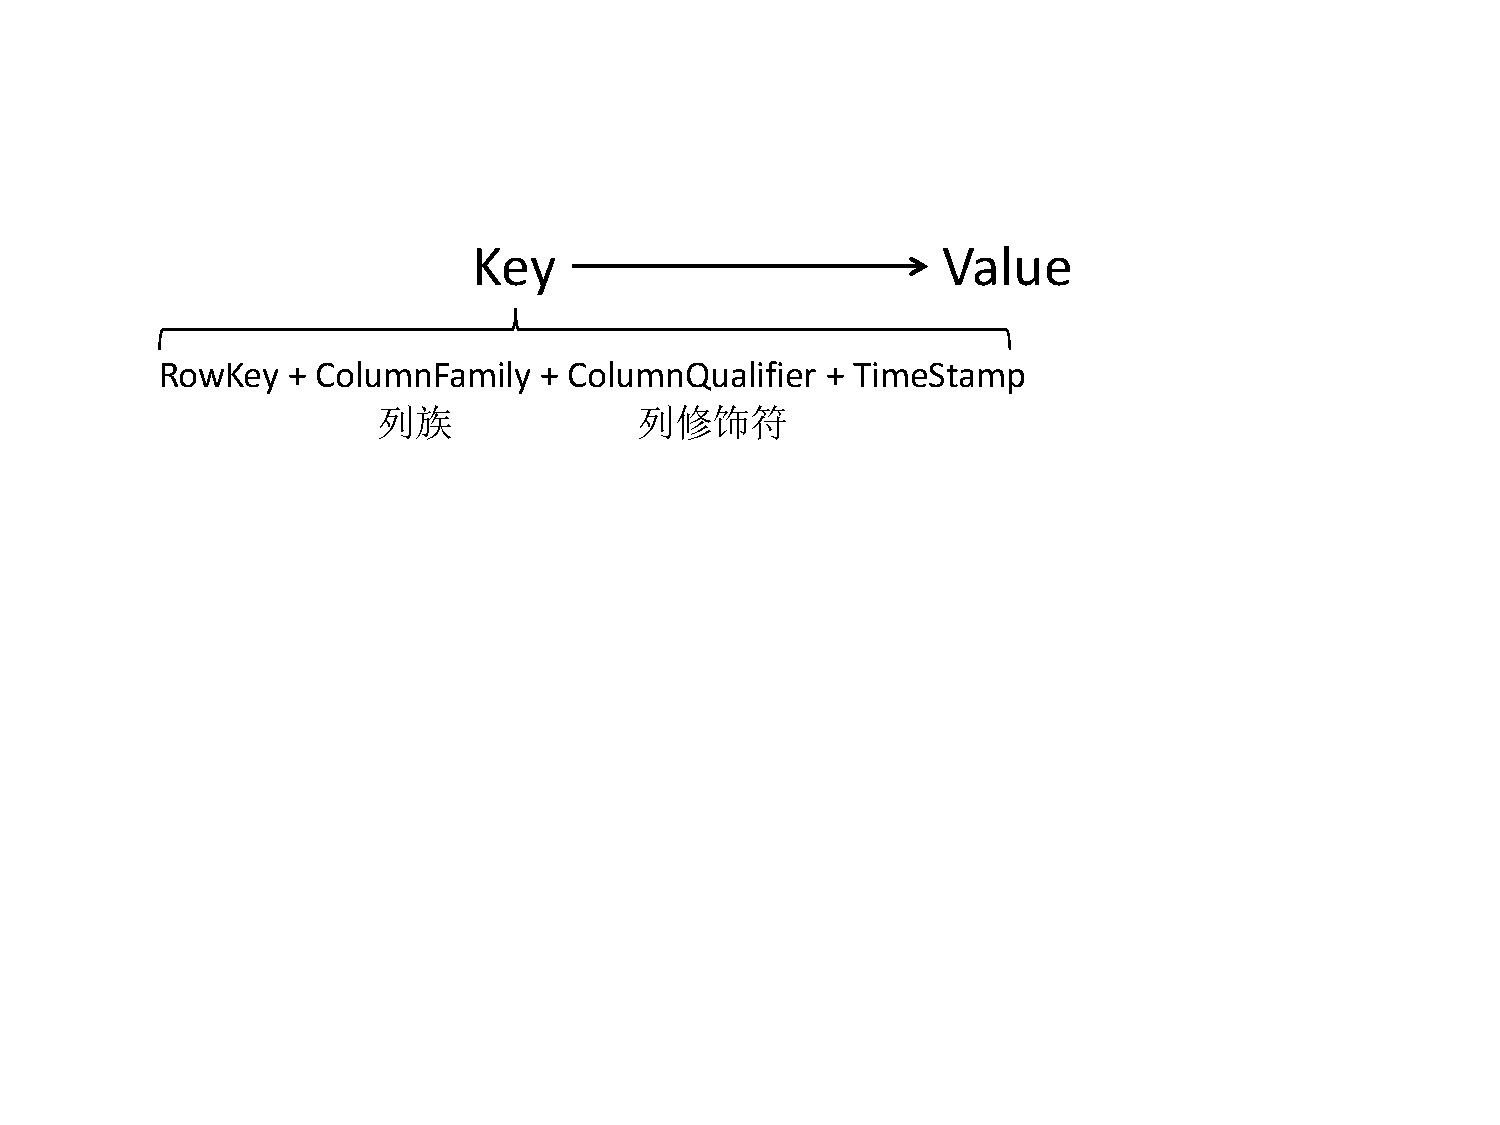
\includegraphics[width=120mm]{fig/HBase_key_value.pdf}
\caption{HBase中Cell单元的Key、Value成分}
\label{fig:hbase_cell}
\end{figure}

\subsection{HBase操作接口}
HBase提供了一个交互式的shell作为操作接口,同时也提供原生的Java接口,另外还提供了thrift API,支持C++、Python、Ruby、Perl、PHP等语言。下面以HBase shell为例叙述HBase的操作接口。

HBase建表时需要指定表中的所有列族,下面的操作创建了名为table1的数据表,它拥有两个列族cf1和cf2:
\begin{lstlisting}
HBase Shell > create 'table1', 'cf1', 'cf2'
\end{lstlisting}

在建表之后还可以增加或删除列族,也可以修改列族的配置,但需要disable整个表,即中止所有读写请求,操作结束后再enable该表:
\begin{lstlisting}
HBase Shell > disable 'table1'
HBase Shell > alter 'table1', {NAME => 'cf2', VERSIONS => 5}
HBase Shell > alter 'table1', 'delete' => 'cf1'
HBase Shell > alter 'table1', 'cf3'
HBase Shell > enable 'table1'
\end{lstlisting}
上面的操作设置列族cf2的最大版本数为5,即每列最多存储5个版本的数据。下一行删除列族cf1及其下的所有数据。之后添加一个列族cf3。

HBase提供Put、Get、Scan、Delete接口进行数据的增删查改。Put接口给某一行中插入一个单元格,需要指定行键、列族和列修饰符。时间戳则是可选的,若没有指定,则使用插入时间作为时间戳。
\begin{lstlisting}
HBase Shell > create 'table1', 'cf1', 'cf2'
HBase Shell > put 'table1', 'row1', 'cf1:a', 'value1'
HBase Shell > put 'table1', 'row2', 'cf2:b', 'value2'
HBase Shell > put 'table1', 'row1', 'cf1:b', 'value3', timestamp1
\end{lstlisting}

Delete接口跟Put接口相反,用来删除一个单元格的数据。由于参数相同,这里不再举例。

Get接口跟Scan接口用来读取数据,其中Get接口用来读取一行内的数据,Scan接口用来读取多行的数据。Get接口只需给定一个行键,参数里的列族、列修饰符和时间戳都是可选的,会把满足条件的所有单元格都返回。Get接口能读取的范围不超过一行,即Get接口可以读取一个单元格,也可以读取一行中所有的单元格,但读取的对象都只能在同一行中。下面是一些读取示例:
\begin{lstlisting}
HBase Shell > get 'table1', 'row1'
HBase Shell > get 'table1', 'row1', 'cf2:a'
HBase Shell > get 'table1', 'row1', {COLUMN => ['cf:a', 'cf:b', 'cf:c']}
HBase Shell > get 'table1', 'row1', {COLUMN => 'cf:c', TIMESTAMP => ts1}
\end{lstlisting}

Scan接口则用来读取连续的多行数据。在HBase数据表中各行是按行键升序排列的,因此Scan时只需给定一个起始行键和一个终止行键(不包含),就可以返回所有的这些行。如果不给定范围,则Scan接口返回表中的所有数据。Scan接口也可指定特定的列或附加Filter来过滤无关数据。下面是一些操作示例:
\begin{lstlisting}
HBase Shell > scan 'table1', {LIMIT => 100}
HBase Shell > scan 'table1', {COLUMNS => ['cf1:a', 'cf1:b'], LIMIT => 10,
                              STARTROW => 'xyz'}
\end{lstlisting}
第一行读取表中的100行数据,第二行从行键大于等于'xyz'的行中读取列族为cf1,列修饰符为a或b的10行数据。

之所以要区分Get和Scan接口,是因为HBase只保证单行数据的原子性,即Get接口不会返回部分更新的数据,但Scan接口没有这个保证。
在本节也可以看到,HBase并没有提供类型关系数据库的SQL接口,这是所有NoSQL数据库的一个特点,都是根据自己的数据模型因地制宜地提供对应的接口。

% ACID的支持情况是否要说?

\subsection{HBase存储实现}
HBase集群采用Master-Slave架构,其中Master节点为HMaster,Slave节点为RegionServer,每台工作机器只需部署一个RegionServer。
HMaster和RegionServer之间通过ZooKeeper\footnote{ZooKeeper, http://zookeeper.apache.org/}来协同工作。HMaster没有单点问题,HBase中可以启动多个HMaster,通过Zookeeper的Master Election机制保证总有一个HMaster在运行。

\begin{figure}[htbp]
\centering
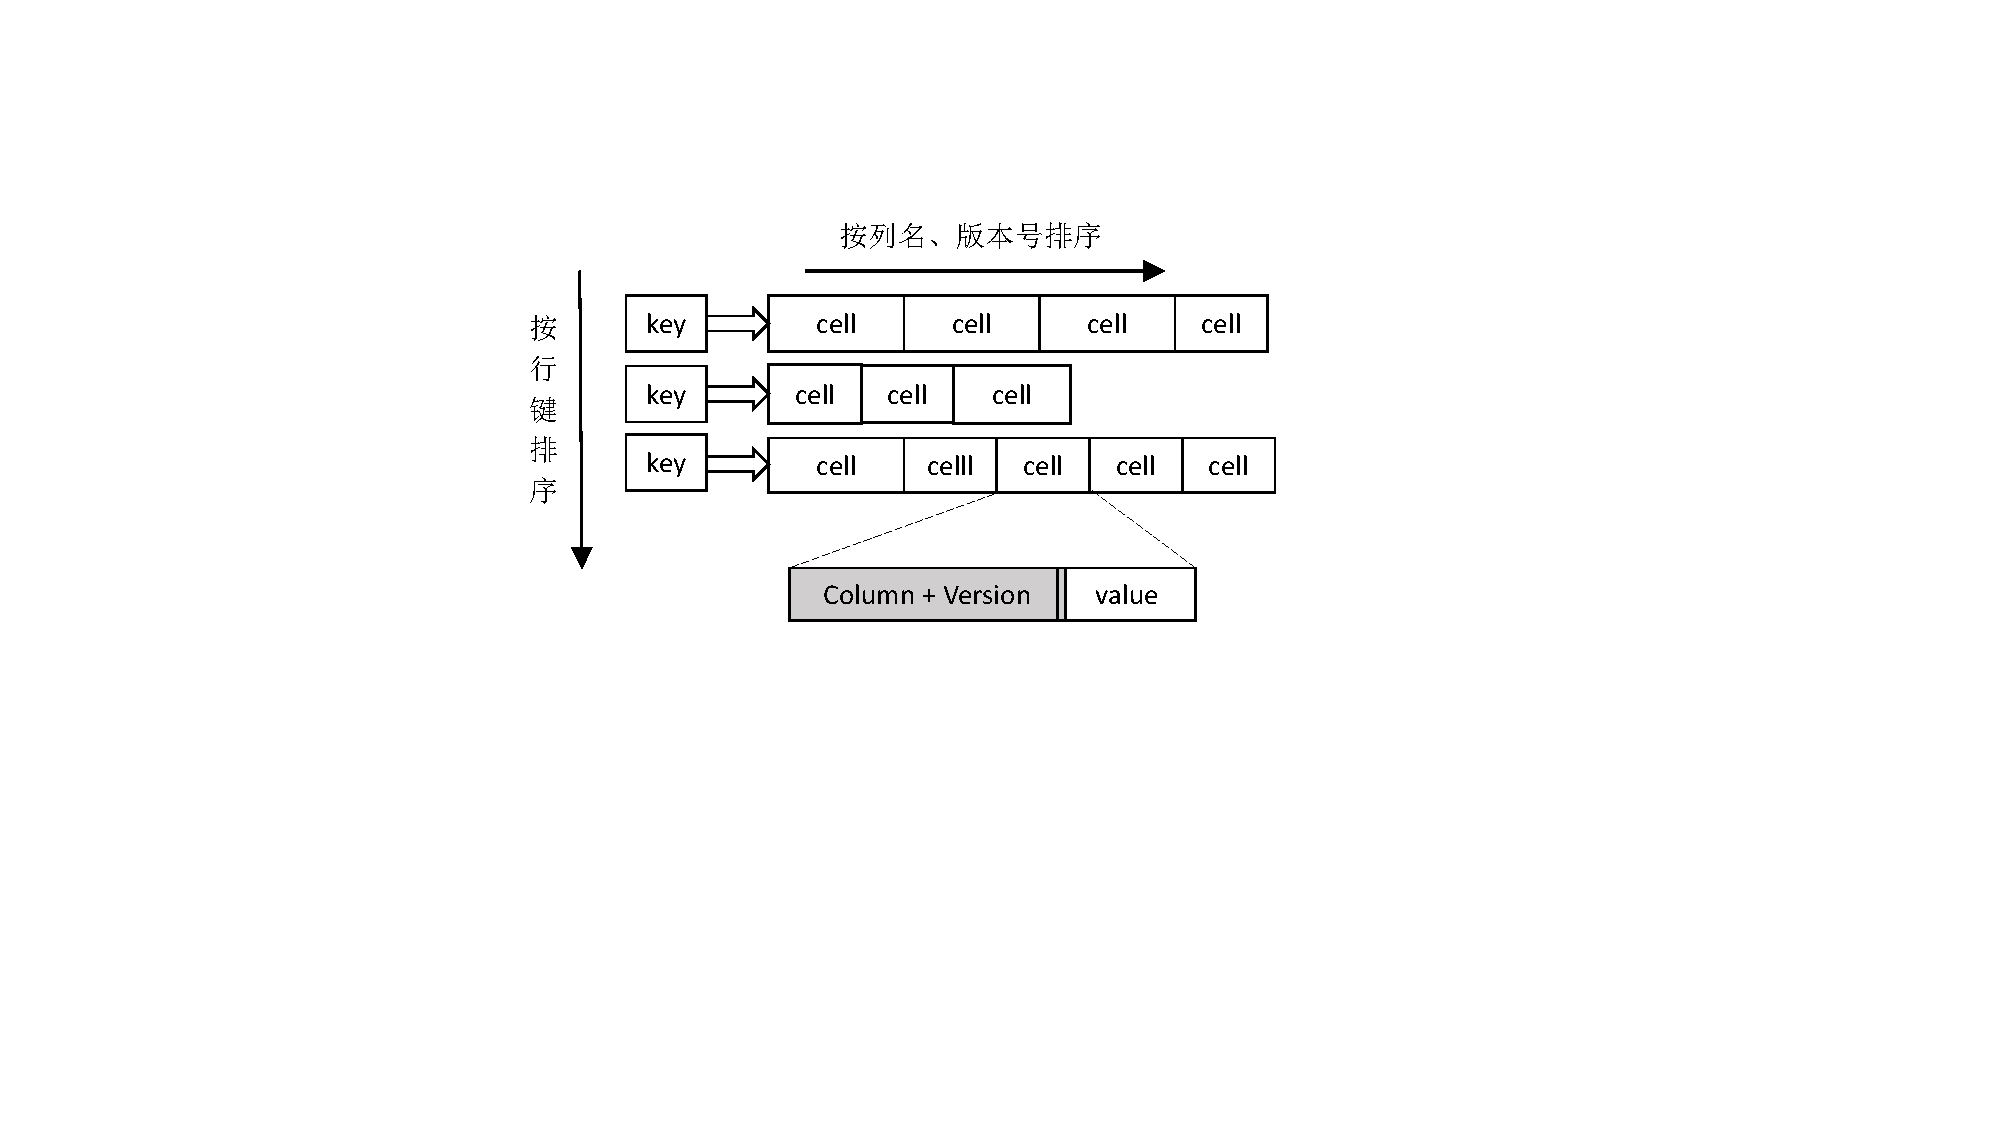
\includegraphics[width=100mm]{fig/big_table.pdf}
\caption{BigTable模型示例}
\label{fig:big_table}
\end{figure}

RegionServer负责管理数据表的分片(Region)。HBase采用BigTable数据模型(如图\ref{fig:big_table})。在BigTable数据表中,各行首先按行键升序排列,行内的各单元格再依次按列名、时间戳排序。作为一个列式存储数据库,HBase中不同列族的数据是分开存储的。由于行键有序,因此可以装数据表水平切分为不相交的Region,每个Region由一个左闭右开的行键区间来表示。每个Region交由一个RegionServer来管理,RegionServer进一步将这些数据存储在HDFS中,并响应这个Region上的读写请求。

\begin{figure}[htbp]
\centering
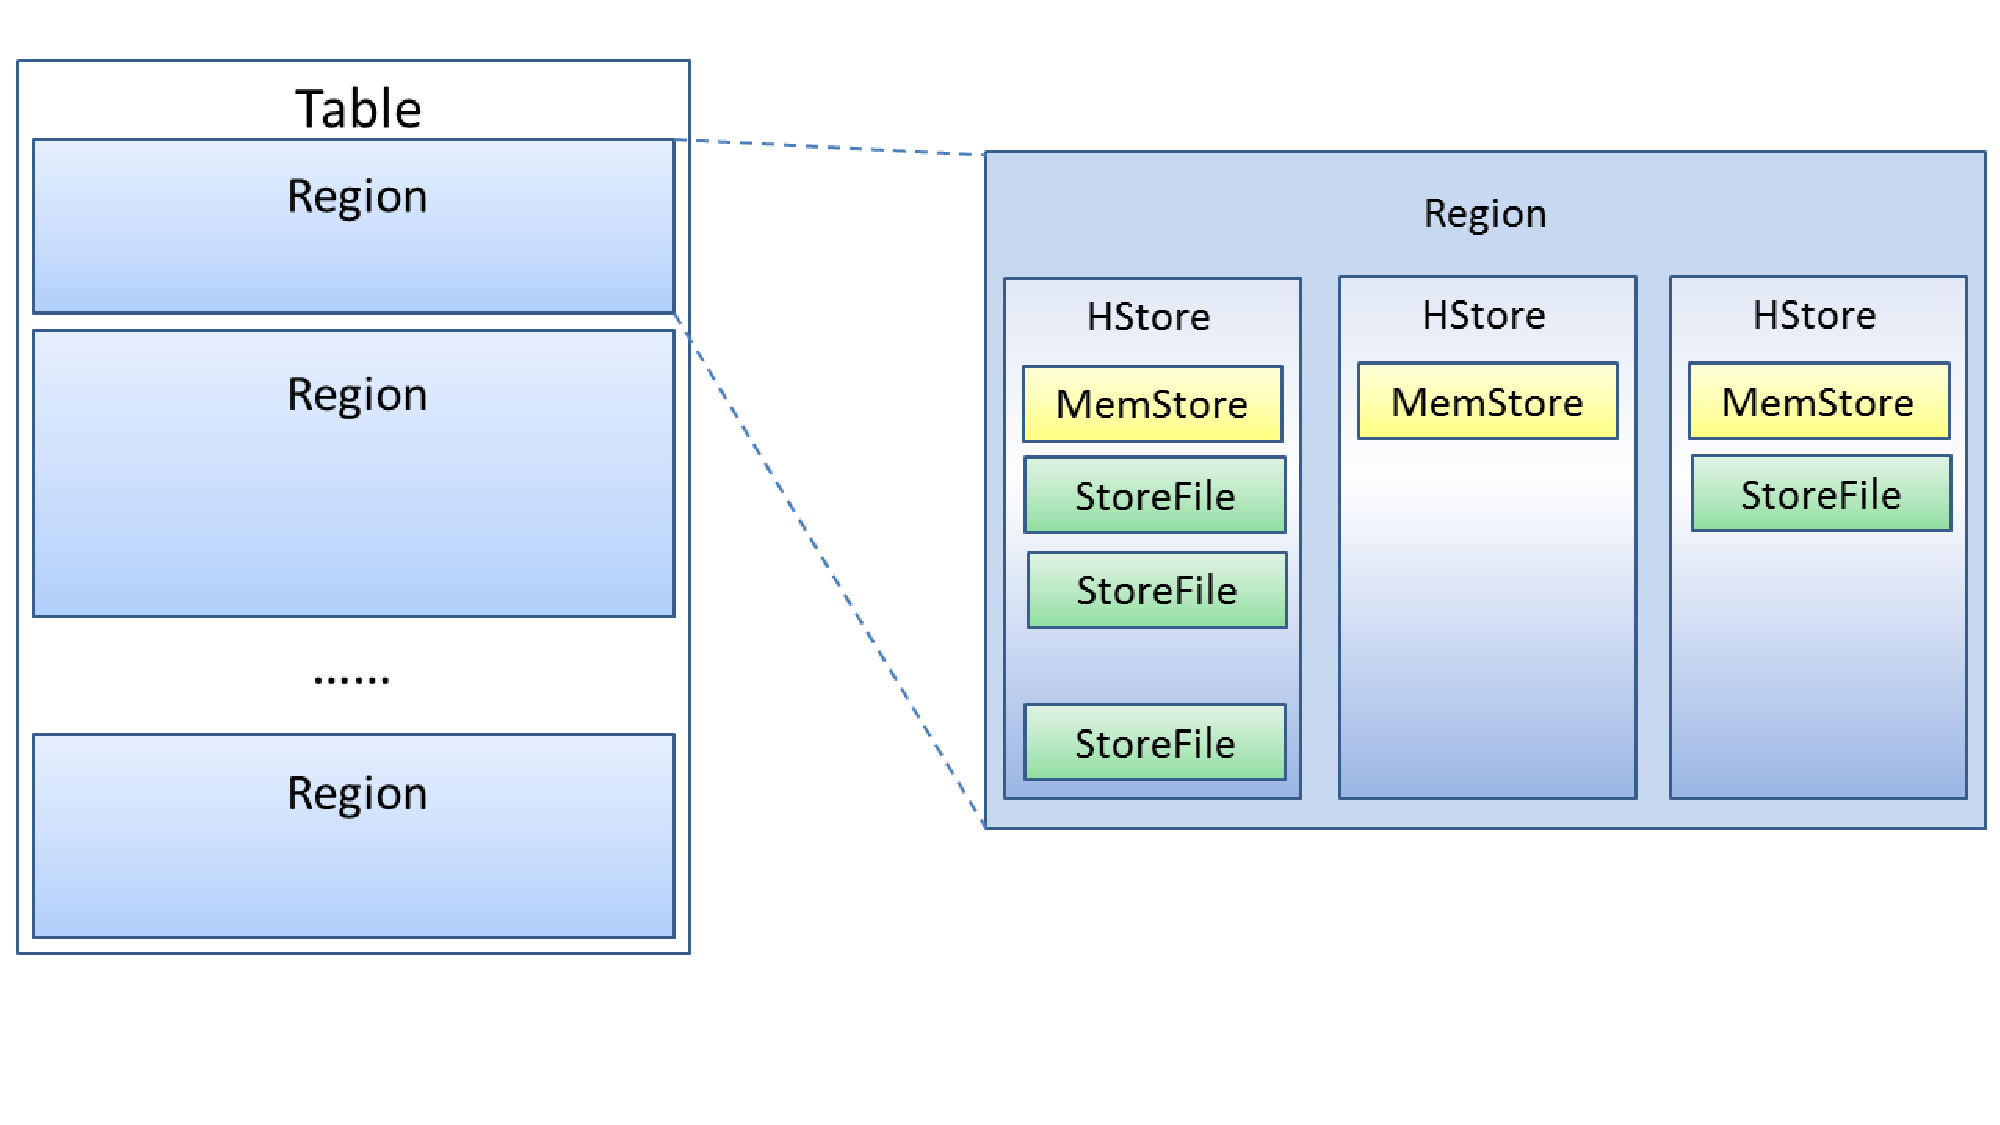
\includegraphics[width=120mm]{fig/HBase_region.pdf}
\caption{HBase Region内部结构}
\label{fig:hbase_region}
\end{figure}

每个Region在RegionServer内的组成成分如图\ref{fig:hbase_region}所示。
Region内部先按列族分为不同的HStore,每个HStore采用LSM Tree\supercite{LSM_tree}数据结构进行存储。在LSM Tree中,数据更新先写入内存缓冲区MemStore中,在MemStore中数据是有序排列的。当MemStore写满时,会将数据flush进磁盘成为文件,即一个StoreFile。由于生成StoreFile时是磁盘的顺序写,因此具有很高的性能。HBase利用LSM Tree数据结构实现了高效的随机写入。然而给定一个Key值要进行读取时,需要在MemStore和所有StoreFile中进行查找,如果StoreFile数目过多将会影响读取速度。RegionServer有线程会定期对HStore里的StoreFile进行合并(compaction),以降低StoreFile的数目,减小读请求的开销。

最后需要补充的是,每个RegionServer会维护一个WAL(Write Ahead Log)文件,写请求在写入MemStore前都需要先写入WAL中,以保证宕机时内存中的数据不会丢失。WAL和底层的StoreFile都是存储在HDFS上的,具有多复本的容错机制。当某台 RegionServer 宕机时,HMaster会将这些文件分配给其它RegionServer进行恢复,从而实现容错性(Fault Tolerance)。

\subsection{HBase与同类系统对比}
在分布式键值存储中,另一个著名的系统是Cassandra\supercite{cassandra}。Cassandra是Amazon DynamoDB\supercite{DynamoDB}的开源实现,最初由Facebook开发并开源。

在存储实现方面,区别于BigTable中按字典序来划分Key值空间的实现,Cassandra中是按Key值的哈希值来划分空间的。另外Cassandra不依赖于HDFS进行存储,其数据直接由各Server存储在本地磁盘中,Server之间对数据保留多个复本。由于Key值的寻址逻辑更为简单,以及更为直接的存储实现,Cassandra相比HBase具有更优的读写性能。

在系统架构方面,Cassandra使用去中心化的系统架构,没有Master节点,因此完全除去了单点故障的可能。所有Server组成一个环状结构,使用一致性哈希算法来分配Key值空间。一致性哈希算法使得集群可以方便地添加或删除节点。区别于HBase依赖ZooKeeper进行协作,Cassandra中的Server之间使用Gossip协议进行协作。

Cassandra与HBase最大的区别在于CAP\supercite{CAP}理论上的取舍。CAP是Consistency、 Availability、 Partition tolerance的简称,表示分布式系统的三个性能。Consistency是指系统的读请求总能返回最新的写结果,即读写请求是一致的。Availability是指系统一直处于可用的状态,不会因为宕机等原因造成一段时间不可服务。Partition tolerance是指分布式系统因网络故障等被切分为不可通信的几部分时仍能正常工作。CAP理论指出,任何系统最多只能满足三条性能中的两条,不可能三者兼备。

HBase和Cassandra都是分布式的系统,在部分机器宕机或失联时系统仍能工作,都是满足Partition tolerance的。它们的区别在于Consistency和Availability的取舍上。
HBase 在有RegionServer宕机时,需要让相应的WAL和StoreFile在其它RegionServer上进行恢复,在恢复期间对应的Region是无法提供服务的,因此不满足Availability。但也正得益于这种恢复机制,HBase中的数据会一直处于一致的状态,即HBase满足Consistency。
Cassandra由于不依赖HDFS之类的可靠存储层,需要自身在各Server间对数据做多复本存储。而读请求是可以由单独一台Server来响应地,不需要等待各Server间的同步,因此也就没有了一致性的保证,按来了读写的高性能。

\section{图数据库Titan}
图数据库是以图的形式来表示和管理数据的数据库\supercite{graph_models_survey},与传统的关系型数据库相比,图数据库在图结构相关的查询上有更优异的性能,如多跳邻域查询、路径查询、局部聚集系数计算等。
Titan是一个基于Blueprints\footnote{Blueprints, https://github.com/tinkerpop/blueprints/wiki} 接口设计的开源图数据库。Blueprints是属性图数据库的一套标准,类似于关系数据库里的JDBC,大部分图数据库都实现了Blueprints接口。

\begin{figure}[htbp]
\centering
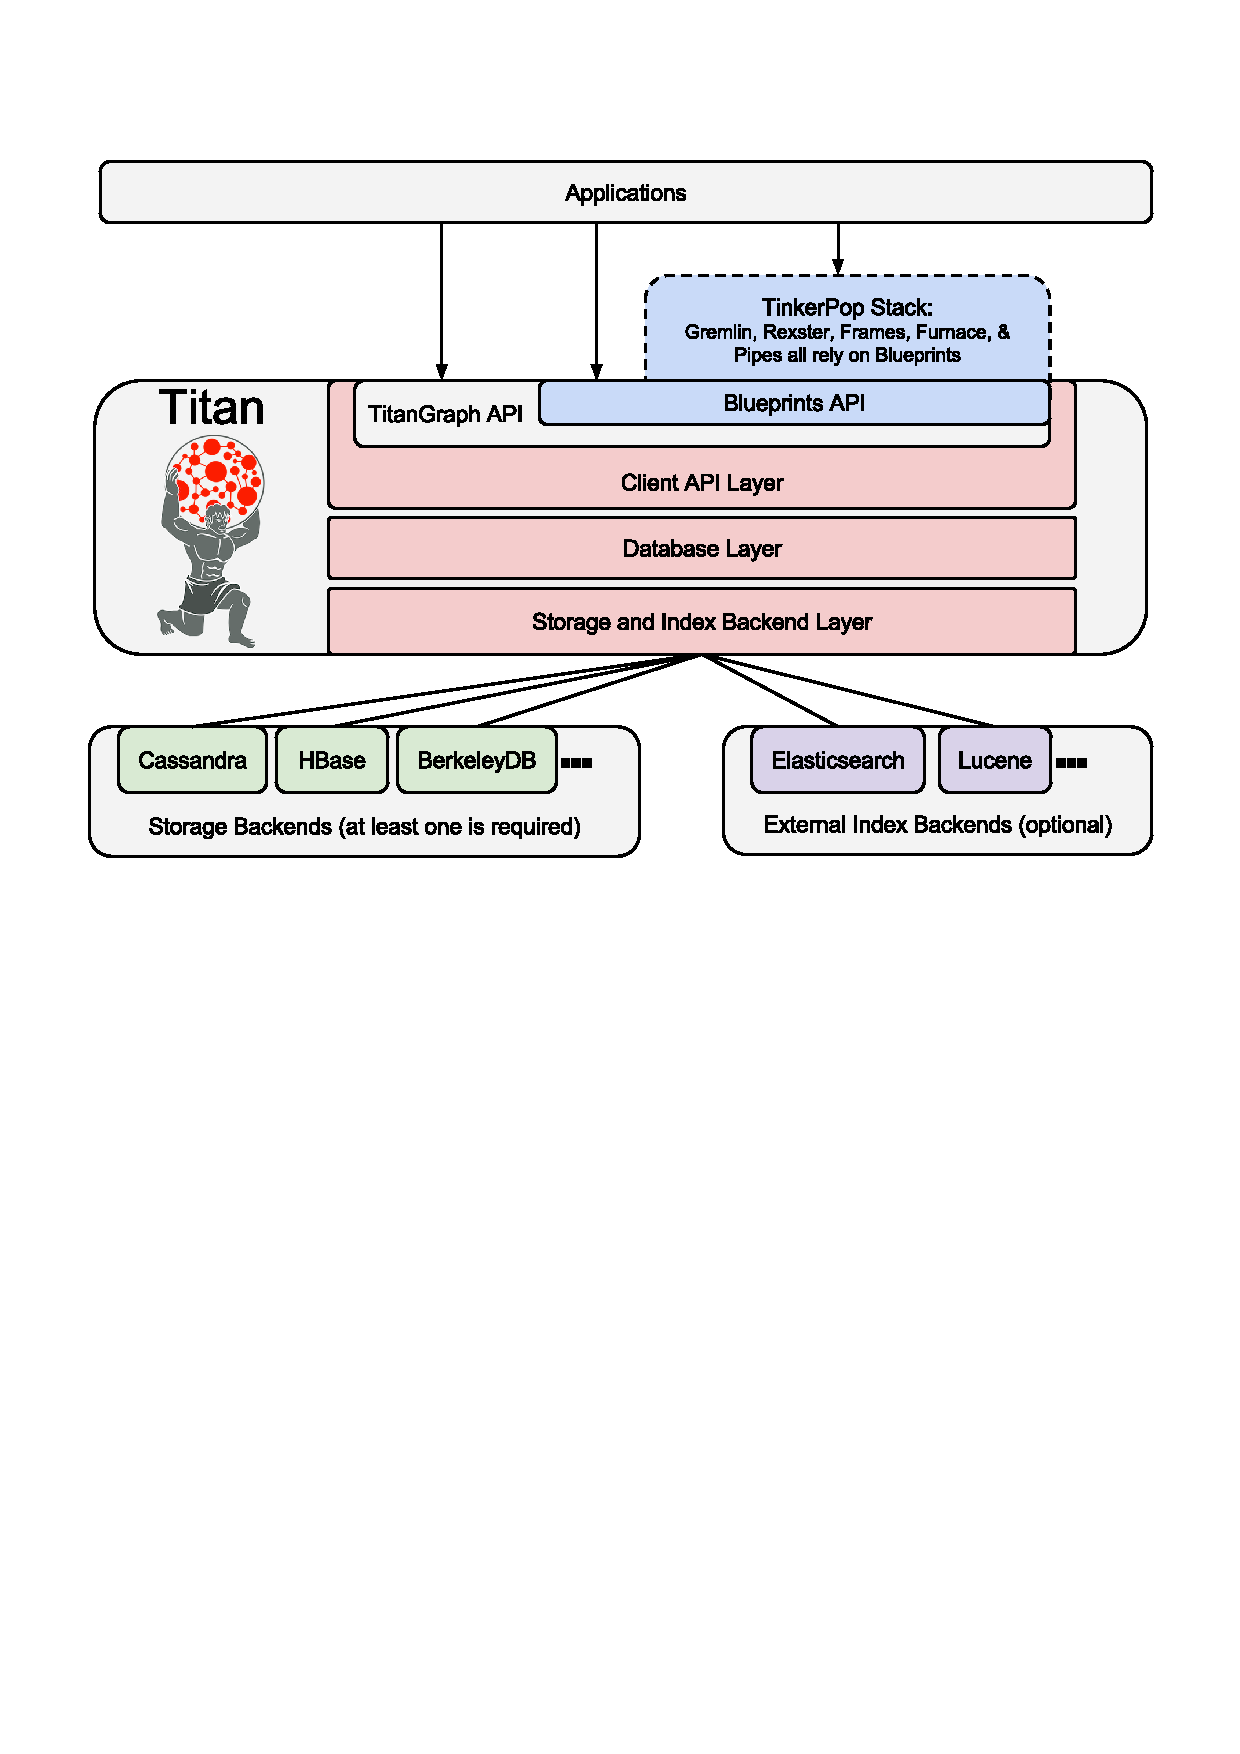
\includegraphics[width=140mm]{fig/titan-architecture.pdf}
\caption{Titan架构图}
\label{fig:titan_arch}
\end{figure}

Titan实现了可插拔的存储接口,可以部署在BerkerlyDB 、HBase或Cassandra之上 ,即Titan不会自己管理数据,其数据存储在底层的存储引擎之中。Titan在索引方面也提供了可插拔的接口,因为Titan只利用存储引擎实现了精确匹配的索引(类似倒排索引),更高级的索引需要依赖索引引擎来实现。Titan支持的索引引擎有ElasticSearch、Lucene等。图\ref{fig:titan_arch}是Titan架构图\footnote{图片来源:http://s3.thinkaurelius.com/docs/titan/0.5.4/images/titan-architecture-layer-diagram.svg}。

相比于著名的图数据库Neo4j,Titan是完全开源免费的,其受关注度正在与日俱增。而且由于Hadoop生态系统在产业界的广泛应用,在HBase上搭建Titan,即使用Titan on HBase应对图处理需求是较为常见的选择。下面分别介绍Titan的操作接口、Titan的存储实现,以及Titan在处理大量重边时的局限性。

\subsection{Titan操作接口}
\subsubsection{Schema设置(DDL接口)}
图的Schema包括edge labels、vertex labels和property keys等。Property key是指某种属性的Key值,如"name"、"gender"、"age"等。label是点和边的标签,可以认为是一种特殊的属性,但每个元素只能有一个label。这些都需要在使用前事先定义。

定义点的label只需要给定一个label名,后续在添加点时,需要指定使用的是哪个vertex label。下面是操作示例:
\begin{lstlisting}
mgmt = g.getManagementSystem()
person = mgmt.makeVertexLabel('person').make();
mgmt.commit()
// Create a labeled vertex
person = g.addVertexWithLabel('person')
// Create an unlabeled vertex
v = g.addVertex(null)
g.commit()
\end{lstlisting}

Edge label的定义需要给出lable名,以及边的重复度限制(Multiplicity)。
Multiplicity 有 MULTI、 SIMPLE、 MANY2ONE、 ONE2MANY、 ONE2ONE 五种取值。其中 MULTI 表示这种类型的边可以在两点间连任意多条,即本文研究的重边。 SIMPLE表示两点间最多只能连一条这样的边,比如好友关系,如果两人之间有好友关系,则连一条这样的边,否则不连。加上 SIMPLE 类型使得两人之间不能连多条表示好友关系的边。MANY2ONE 表示每个点至多只有一条这样的出边,但是对该label的入边数目没有限制。比如表示mother关系(母子关系)的边,一个人只能有一个母亲,但一个母亲可以有多个孩子。 ONE2MANY 的意义与 MANY2ONE 相反,每个点至多只有一条这样的入边。 ONE2ONE 表示这种边是一对一的,即两个点之间如果连了一条这样的边,这两个点就不能再跟任何其它点有这样的边相连。比如夫妻关系,就是 ONE2ONE的 例子。下面是创建edge label的示例:
\begin{lstlisting}
mgmt = g.getManagementSystem()
follow = mgmt.makeEdgeLabel('follow').multiplicity(Multiplicity.MULTI).make()
mother = mgmt.makeEdgeLabel('mother').multiplicity(Multiplicity.MANY2ONE).make()
mgmt.commit()
\end{lstlisting}

Property key的定义需要给出key的名称,以及数据类型,还有数据的基数(Cardinality)。 Cardinality有 SINGLE、 LIST、 SET 三种选择。 SINGLE就是最普通的 key-value对,即value部分只会填一个单一的值。 LIST是指value部分是一个列表,对value部分的操作将是添加或删除部分值。 SET则表示value部分是一个去重的值的集合。下面是一些操作示例:
\begin{lstlisting}
mgmt = g.getManagementSystem()
birthDate = mgmt.makePropertyKey('birthDate').dataType(Long.class).cardinality(Cardinality.SINGLE).make()
name = mgmt.makePropertyKey('name').dataType(String.class).cardinality(Cardinality.SET).make()
sensorReading = mgmt.makePropertyKey('sensorReading').dataType(Double.class).cardinality(Cardinality.LIST).make()
mgmt.commit()
\end{lstlisting}

\subsubsection{查询接口}
Titan提供Gremlin\footnote{Gremlin, https://github.com/tinkerpop/gremlin/wiki}查询接口让用户可以在图上进行游走(traversal)查询。Gremlin是基于Blueprints接口实现的一门函数式图查询语言,可以把图查询表示成链式的函数调用,使得代码非常直观。

下面是一个查询示例,查询 name 属性为 hercules的点在 father关系上两跳出边的点的 name属性值。
\begin{lstlisting}
gremlin> g.V.has('name','hercules').out('father').out('father').name
==>saturn
\end{lstlisting}

下面是一个更丰富的查询示例,在找到name为hercules的点后,查询其father、mother出边连接的点的label,查询结果为'god'和'human'。再查询hercules节点所有battled出边所连接的点的label,查询结果是3个邻接节点的label都为monster。最后一个查询显示所有battled出边所连接的点的所有属性。每个点只有一个key值为name的属性,因此每行中只有一个key value对。
\begin{lstlisting}
gremlin> hercules = g.V.has('name','hercules').next()
==>v[1536]
gremlin> hercules.out('father','mother')*.getVertexLabel()
==>god
==>human
gremlin> hercules.out('battled')*.getVertexLabel()
==>monster
==>monster
==>monster
gremlin> hercules.out('battled').map
==>{name=nemean}
==>{name=hydra}
==>{name=cerberus}
\end{lstlisting}

Gremlin也可以表达一些复杂的查询条件,如给定两个点v1和v2,查询它们之间的所有边:
\begin{lstlisting}
gremlin> v1.bothE   // get all edges of v1
gremlin> v1.bothE.filter{it.outV.next() == v2 || it.inV.next() == v2}
\end{lstlisting}
第一行的查询将返回v1的所有出边和入边。第二行的查询则在所有边的基础上加了个filter,接收一个表达式(Closure)作用在迭代器上,迭代器it每次指向一条边,判断它的端点是否包含v2,如果包含则表明是v1和v2共用的边。因此第二行返回v1、v2相连的所有边。


\subsubsection{数据操作接口(DML接口)}
用Gremlin在图中插入点和边是很方便的,下面是一个插入数据的示例:
\begin{lstlisting}
alice = g.addVertexWithLabel("person")
alice.setProperty("name", "Alice")
bob = g.addVertexWithLabel("person")
bob.setProperty("name", "Bob")

e = alice.addEdge("isFriend", bob)
e.setProperty("since", 1991)
g.commit()
\end{lstlisting}
g是一个TitanGraph对象,第1、2行往图中插入一个label为"person"的点,并设置属性"name" 为"Alice" ,第3、4行类似地插入一个表示Bob的点。第6、7行在这两个点间连一条label为 "isFriend"的边,并设置边上的属性。最后第8行需要执行commit,以将修改持久化到存储中。同时这也表示当前事务的结束,在Titan中,对图(即对象g)的初次操作将打开一个Thread Local的事务,只有执行commit才能结束当前事务。

更详细的Gremlin接口介绍,可参见Gremlin文档\footnote{GremlinDocs, http://gremlindocs.spmallette.documentup.com/}。

\subsection{Titan存储实现}
在图数据库Titan中,基于BigTable模型,数据在HBase中以邻接表的形式存储,如图\ref{fig:adj_list}所示。

\begin{figure}[htbp]
\centering
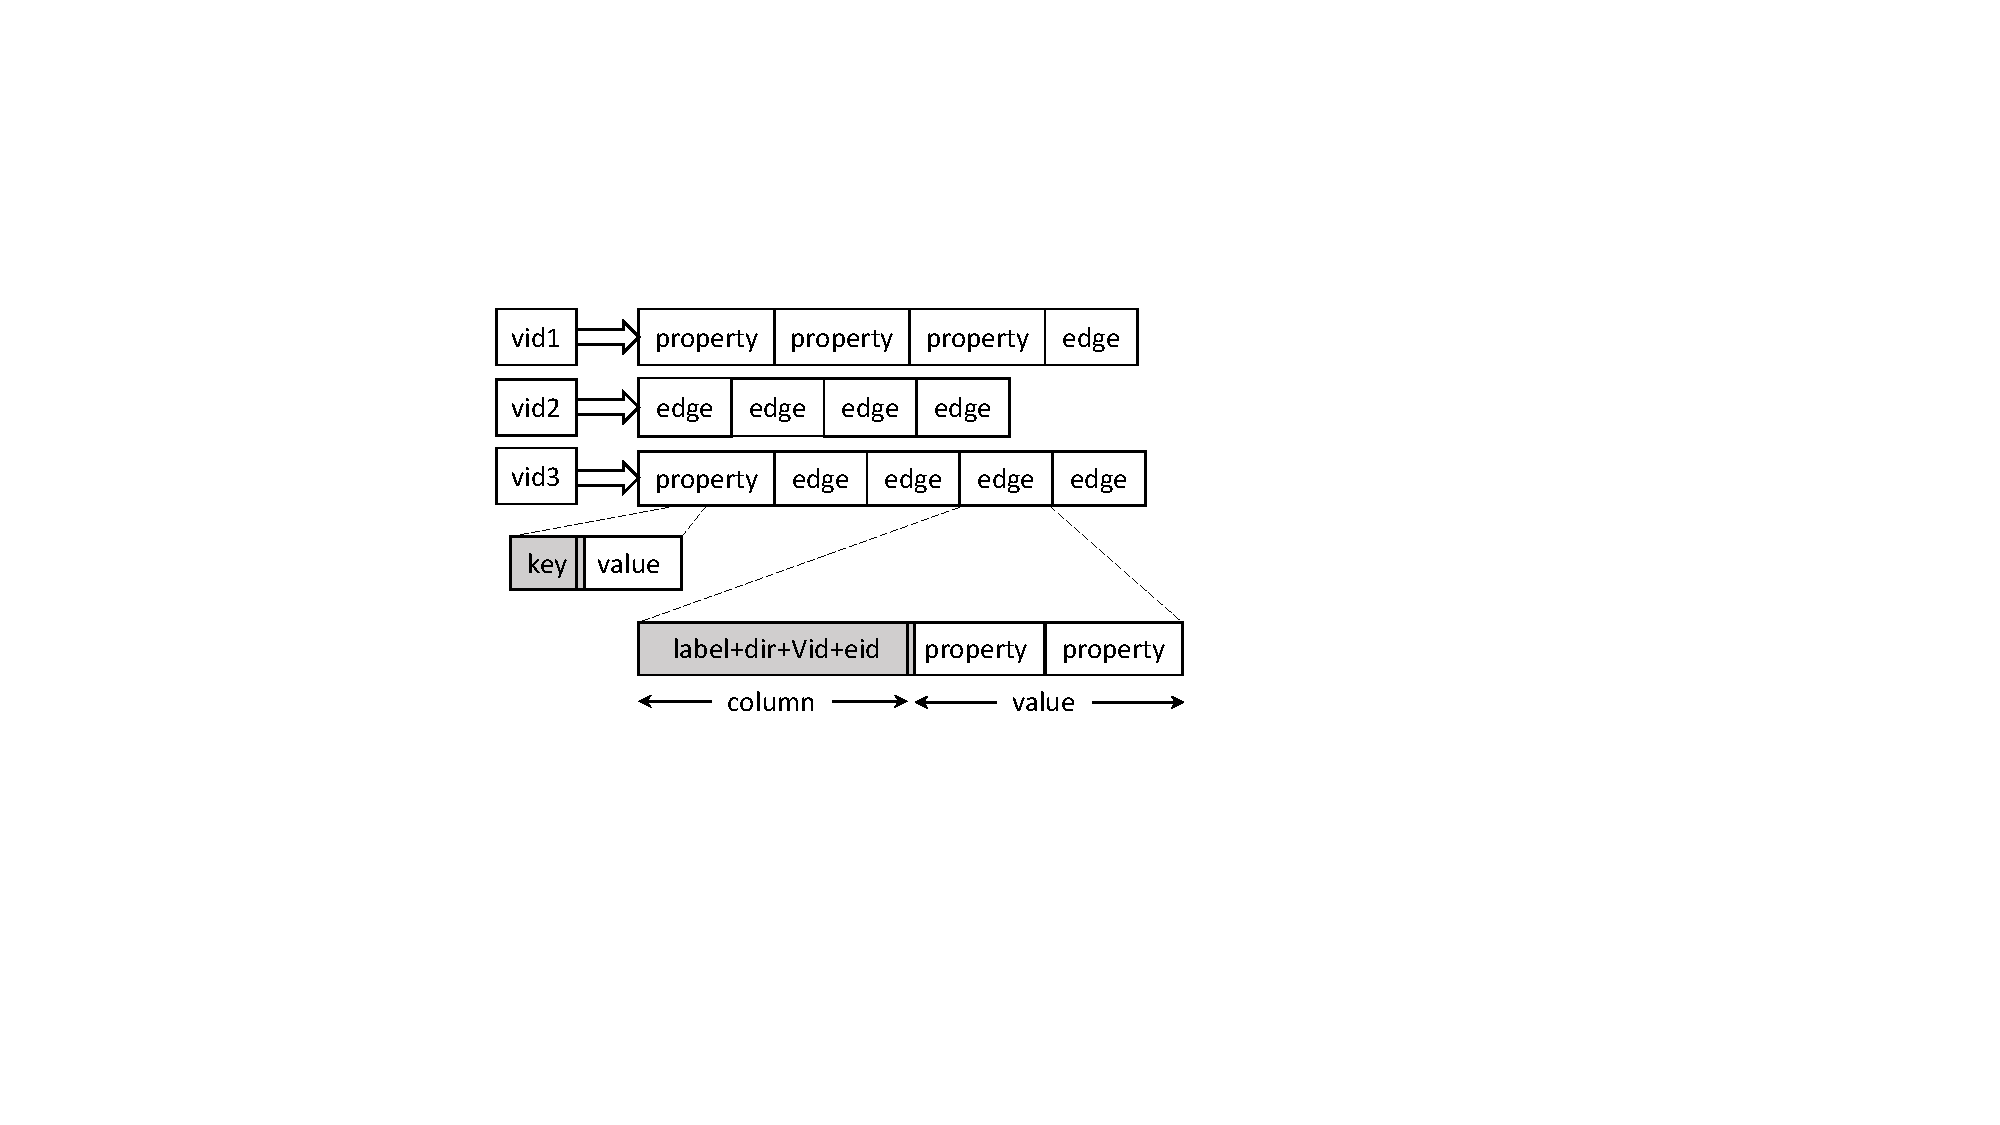
\includegraphics[width=100mm]{fig/adj_list.pdf}
\caption{Titan图数据内部的BigTable表示}
\label{fig:adj_list}
\end{figure}

Titan为每个点分配了一个全局唯一的id,每个点占BigTable中的一行,行键就是点的id。每行存储了该点相关的属性和边,它们各占一个单元格。边和属性数据都存储在一个列族之中,并设置该列族的最大版本数为1,从而使每行中的列修饰符与单元格一一对应,根据行键和列修饰符可以唯一定位到目标单元格,实现对边和属性内容的快速检索。

在Titan中,每个属性是一个key-value对。点的属性存储在该点所在的行,每个属性占一个单元格,并以属性名key作为列修饰符,这使得每个点的属性查询可以非常高效。下面的代码展示了点的属性查询对应的HBase Shell操作,其中"graph\_tbl"是一张图在HBase中的数据表的表名;vid是该点的id,作为行键;边集数据和属性数据所在的列族名为"e"。
\begin{lstlisting}
// Gremlin Command
v.getProperty("name")
// HBase Shell Command
hbase shell> get "graph_tbl", vid, "e:name"
\end{lstlisting}

每个点所在的行还存储了邻接的所有边数据,每条边占一个单元格。一条边的信息包含了邻接点、类别(label)、方向、边的唯一id,以及边上的各属性。单元格的值用来存储边上的所有属性,列修饰符则存储边上除属性外的其它信息。在BigTable模型中,同一行的单元格按列名排序。为了方便检索,每条边所在的单元格依次以label、方向、邻接点id以及边id拼接成为列名,即
\begin{equation}
  \mbox{列修饰符} = \mbox{边}label + \mbox{方向} + adjVid + eid \label{eq:cq_design}
\end{equation}
这种列名设计使得一个点的所有边先按label排序,再按方向、邻接点id、边id等排序。其优点是当要检索该点指定label的所有边时,只需要扫描邻接表的一部分。图\ref{fig:orginal_list}是一个更详细的示例。下面的代码展示了点的边集查询对应的HBase Shell操作。

\begin{lstlisting}
v.getEdges()
hbase shell> get "graph_tbl", vid
hbase shell> // filter out property results

v.getEdges(Direction.OUT, "isFriend")
hbase shell> get "graph_tbl", vid, {FILTER => "ColumnPrefixFilter('isFriend_0')"}

v.getEdges(Direction.BOTH, "isFriend")
hbase shell> get "graph_tbl", vid, {FILTER => 
    "MultipleColumnPrefixFilter('isFriend_0', 'isFriend_1')"}

v1.query().adjacent(v2).edges()
hbase shell> get "graph_tbl", v1_id
hbase shell> // filter results to get only edges with v2_id
\end{lstlisting}

第1行是查询点v的所有边的Titan接口,由于边数据和属性数据都存储在一行中,需要把整行的所有数据读出来(第2行),同时过滤掉属性数据(第3行)。由于点的属性数量和边的数量一般不在一个量级,因此多读入的属性数据的开销不大。

第5行查询点v的所有label为"isFriend"的出边,第6行是其对应的HBase操作。由于给定了label和方向,因此可以知道列修饰符的前缀(根据式\ref{eq:cq_design}),因此从HBase中抽取的数据正好就是所需的边数据。

第7行查询点v的所有label为"isFriend"的边,这里不限定方向,第8、9行是对应的HBase查询。同上一个示例,这里的边有两个方向,可以加两个前缀过滤。

第11行是查询点v1和v2间的所有边,由于邻接点的id在列修饰符中的位置排在label和方向之后(根据式\ref{eq:cq_design}),因此没法给出高效的前缀查询,只能从HBase中把整行的数据抽取出来,再解析过滤出对应v2的所有边。这也正是Titan在边集查询上的局限性,下面将详细讨论。

\subsection{图数据库Titan的局限性}
Titan的邻接表列名设计(式\ref{eq:cq_design}),对于从给定点出发的查询,虽然能高效地查询出某种label的边,但当指定邻接点时,边集查询不得不在底层存储中抽取所有边的数据进行解析过滤(如上节最后的例子)。当图中的重边数量巨大时,Titan的邻接表列数也急剧变大,邻域中点和边的查询性能会急剧下降。

\begin{figure}[htbp]
\centering
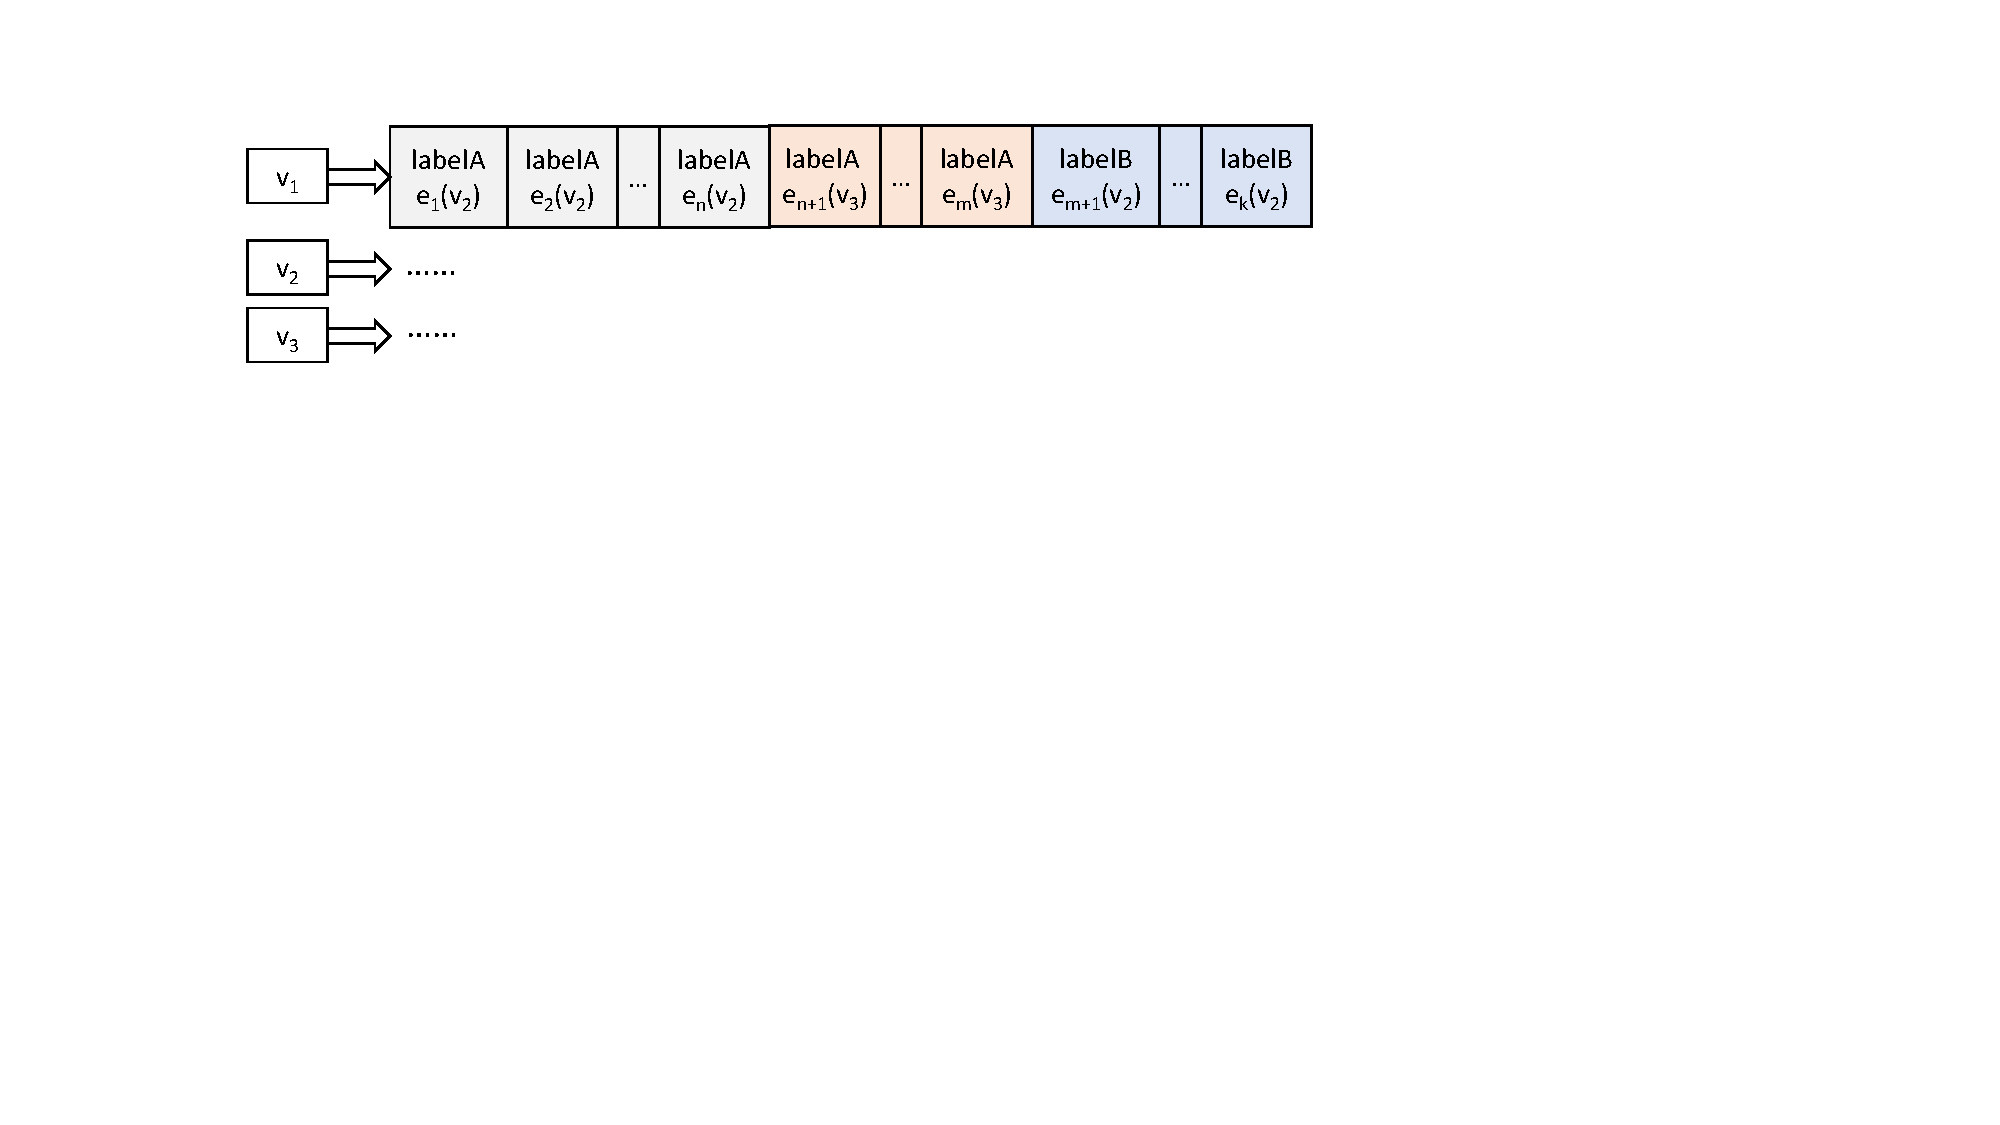
\includegraphics[width=150mm]{fig/original_list.pdf}
\caption[存储大量重边时的邻接表]{当属性图富含重边时,Titan在HBase中的数据表是一张扁平而宽的表}
\label{fig:orginal_list}
\end{figure}

图\ref{fig:orginal_list}展示了富含重边时邻接表的示例,为方便展示省略了边的方向。v1只有v2和v3\\
两个邻接点,其中与v2有两种label的边,与v3有一种label的边。虽然邻接的点数不多,但v1与邻接点都有数量巨大的重边。由于邻接表存储的是每条边的信息,当要查询v1的所有邻接点集(即v2、v3)时,不得不遍历一次v1的所有边,即遍历整行数据。类似地,如果要查询v1与v2的所有边时,由于这些边存储位置不相邻,也只能遍历整行数据再做过滤。

为了规避上述情形,我们可以换一种列名设计来优化邻域点集查询,比如让邻接表先按邻接点id排序,令
\begin{equation}
  \mbox{列修饰符} = adjVid + \mbox{边}label + \mbox{方向} + eid \label{eq:cq_redesign}
\end{equation}
上式与式\ref{eq:cq_design}的区别是把邻接点id(adjVid)移到了第一部分,对应的邻接表变为图\ref{fig:redesign_list}所示。此时优先按邻接点来排序,其次再按边label进行排序。因此邻接点为v2的边现在都排在了一起,可以通过一次scan全部读取出来,不需要再读取整行数据。这样在查询邻接点时,还可以跳过相同邻接点的所有边,不用再遍历整个邻接表。

\begin{figure}[htbp]
\centering
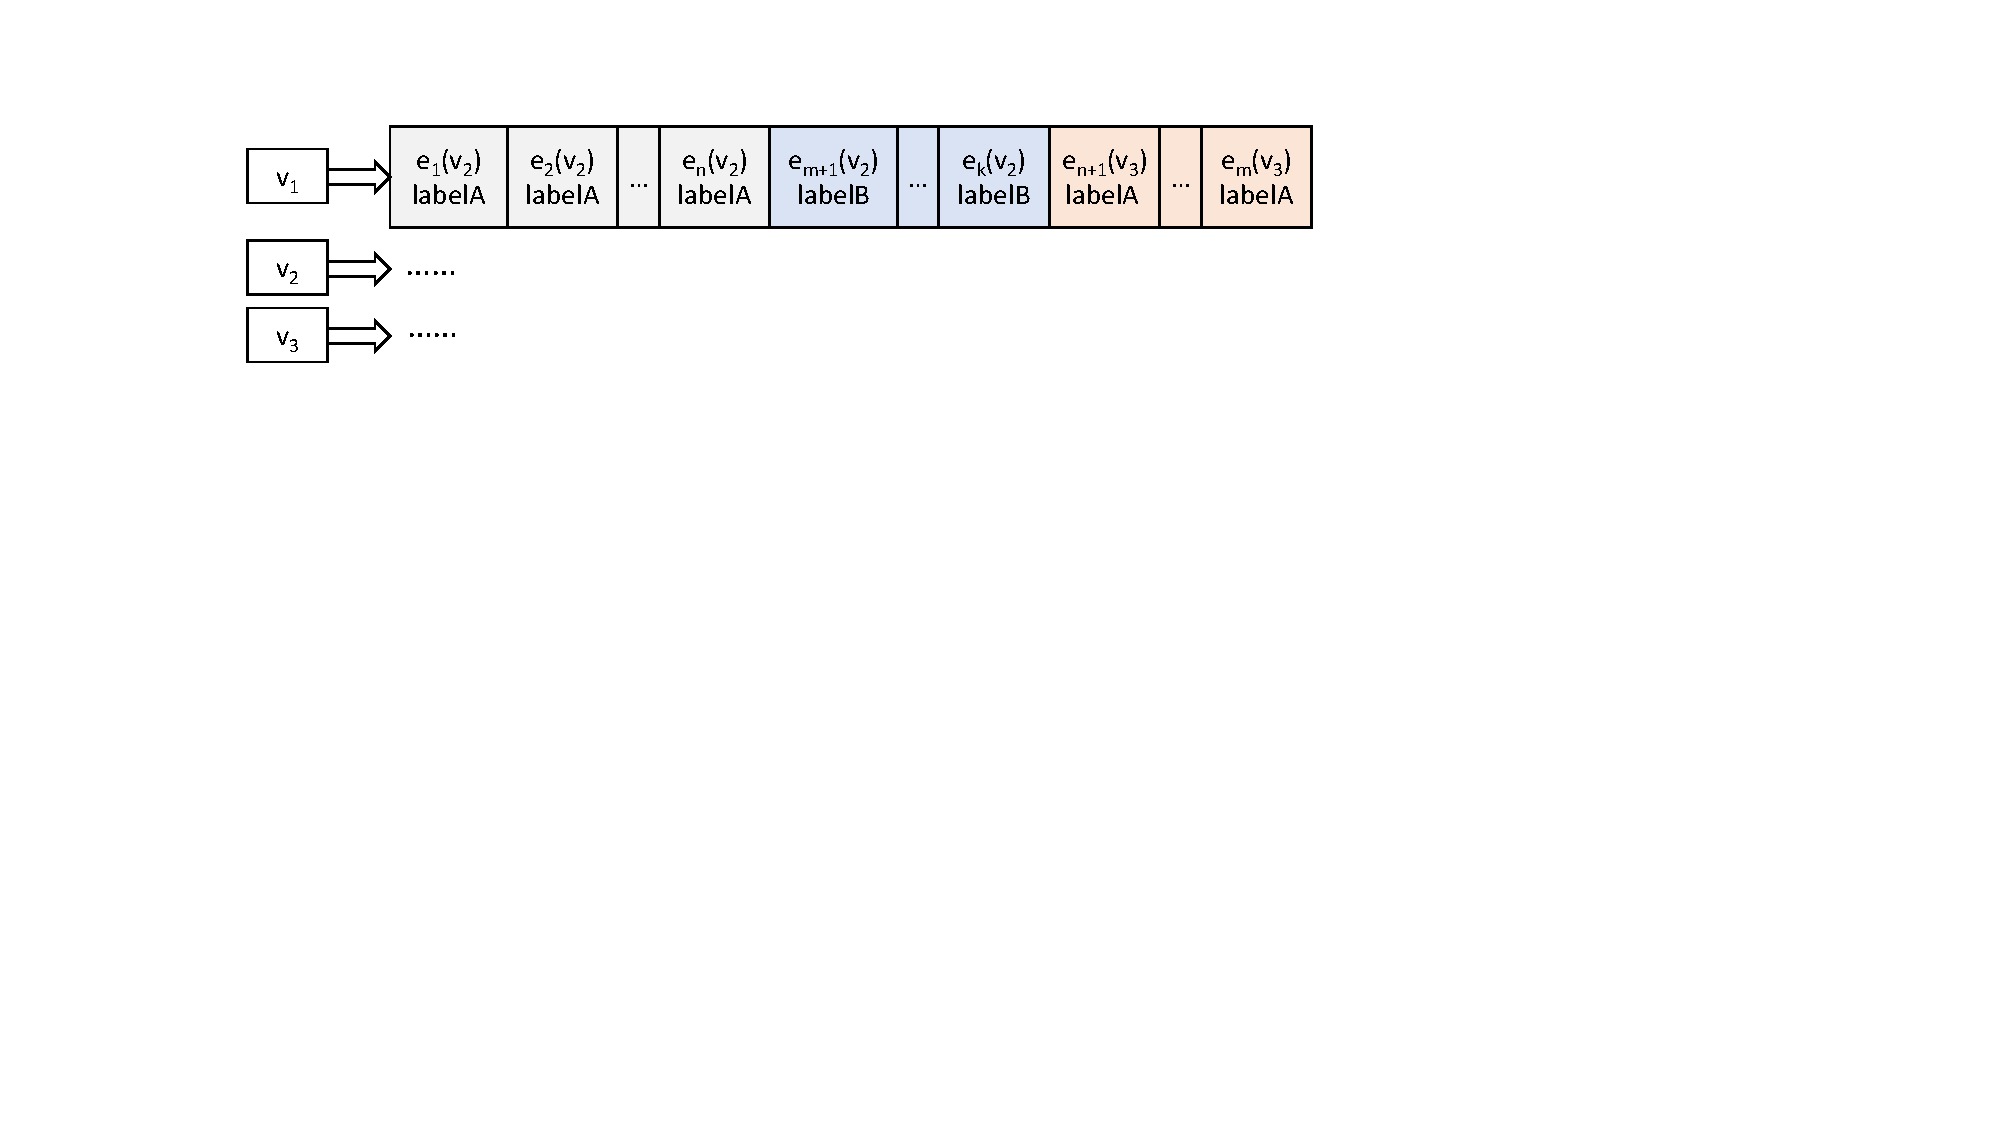
\includegraphics[width=150mm]{fig/redesign_list.pdf}
\caption{重新设计的列修饰符对应的邻接表示例}
\label{fig:redesign_list}
\end{figure}

然而,面对label相关的查询时又会面临同样的问题,比如查询该点总共有几种label的边,或者查询该点某种label的边,仍会面临原来的情形,需要遍历该点的整个邻接表。因此,改变邻接表的列名设计并不能解决问题,本质原因是邻接表存储了所有的边集。不管如何设计列修饰符,对于限定条件不包含列修饰符首位的查询,都需要遍历整行数据再进行过滤。


另一方面,当重边数量巨大时,Titan缓存的低效也影响了查询速度。Titan为加快数据访问设计了缓存,存储最近访问的点及其邻接表内容。其缓存基本上是基于HBase的 Server端Cache来实现的,即最近访问的内容会缓存在RegionServer的 BlockCache中。如果图中各点的重边都很多,则缓存空间被大量的重边占满。然而这些数据经常是与查询结果无关的被过滤数据,在做邻域相关查询时就会极大增加缓存的失效率。

\vspace{2mm}

综上总结如下,Titan在处理大量重边时查询性能急剧下降,主要原因有两方面:
\begin{enumerate}
    \item 不管列修饰符如何设计,总可以找到限定条件不包含列修饰符首位的查询,使得查询需要遍历整行邻接表
    \item 缓存中存放了大量与查询结果无关的重边数据,增加了缓存的失效率
\end{enumerate}

\vspace{3mm}

面对富含重边的属性图,把所有边集都存储在邻接表中是Titan查询性能受损的原因所在。本文基于以上分析,提出了一种基于Titan和列式存储数据库HBase的复合架构设计——HybriG。HybriG架构有如下几方面的特点:
\begin{itemize}
  \item 基于Titan和HBase建立存储层,用Titan来存储图的结构信息和点集的属性信息,HBase存储边集的所有属性信息。
  \item 在HybriG中邻接表保持了项数和数据量上的精简,从而能克服上述图数据库的缺点。
  \item 相比于传统图数据库Titan,HybriG在邻域点集相关查询以及边集数据批量导入上具有优异的性能。
\end{itemize}


% vim:ts=4:sw=4
